\subsubsection{Extremwertaufgabe}

\begin{figure}[H]
	\centering
	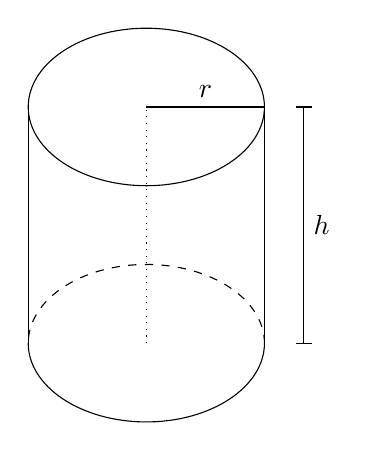
\begin{tikzpicture}
		\draw (1.5,0) arc [start angle=0,end angle=-180,x radius=1.5,y radius=1];
		\draw[dashed] (1.5,0) arc [start angle=0,end angle=180,x radius=1.5,y radius=1];

		\draw (0,3) ellipse (1.5cm and 1cm);
		\draw (-1.5,0) -- (-1.5,3);
		\draw (1.5,0) -- (1.5,3);

		\draw[dotted] (0,0) -- (0,3);
		\draw (0,3) -- (1.5,3);
		\node[above] at (0.75,3) {\( r \)};

		\draw (2,0) -- (2,3);
		\draw (1.9,0) -- (2.1,0);
		\draw (1.9,3) -- (2.1,3);
		\node[right] at (2,1.5) {\( h \)};
	\end{tikzpicture}
	\caption{Skizze Zylinder}
\end{figure}

gegeben: \( V \)

\( O, M \) soll minimal sein

\paragraph{Hauptbedingung}

\[
	O(r, h) = 2 \pi \cdot r^2 + h \cdot 2 \pi r
\]

\paragraph{Nebenbedingung}

\[
	V = h \pi r^2 \Rightarrow h = \frac{V}{\pi r^2}
\]

\paragraph{Zielfunktion}

\begin{align*}
	O(r) & = 2 \pi r^2 + 2 \pi r \frac{V}{\pi r^2} \\
	     & = 2 \pi r^2 + \frac{2V}{r}              \\
	     & = 2 \left(\pi r^2 + \frac{V}{r}\right)
\end{align*}

\begin{align*}
	\frac{\diff 0}{\diff r}                               & = 2 \left( 2 \pi r - \frac{V}{r^2} \right)                            \\
	\frac{\diff 0}{\diff r} (r=r_E) \overset{!}{=} \sigma & = 2 \left( 2 \pi r - \frac{V}{r^2} \right)                            \\
	2 \pi r                                               & = \frac{V}{r^2}                            & \mid \cdot \frac{r^2}{V} \\
	r^3                                                   & = \frac{V}{2 \pi}                                                     \\
	\Rightarrow r                                         & = \sqrt[3]{\frac{V}{2 \pi}}
\end{align*}

\begin{align*}
	\frac{\diff 0}{\diff r} & = 2 \left( 2\pi + \frac{V}{r^3} \right)       \\
	                        & = 2 \left( 2 \pi + \frac{V 2 \pi}{V}  \right) \\
	                        & = 2 (2 \pi + 2 \pi)                           \\
	                        & = 2 (4 \pi)                                   \\
	                        & = 8 \pi > 0 \Rightarrow \text{Minimum}
\end{align*}

\begin{align*}
	h             & = \frac{V}{\pi r^2} \text{ mit } r^2 = \frac{V}{2 \pi r} \\
	\Rightarrow h & = \frac{V}{\pi} \cdot \frac{2 \pi r}{V} = 2r
\end{align*}
